\section{Fusion Energy System Studies}

The objective of this task is to inform the integrated design of fusion energy
systems based on the nuclear, thermo-mechanical and electromagnetic analysis
of individual components of those systems and the systems on the whole.  Two
distinct design concepts, with a number of variations, have been the focus of
consideration by the national \gls{FESS} effort during this performance
period, two variations of ARIES-ACT and a \gls{FNSF}.  The subtasks described
below are arranged according to the broad categories of analysis that are used
to inform any design, rather than by those specific designs.

\subsection{Initial Nuclear Design}

The objective of this subtask is to produce the initial nuclear design, or a
\emph{radial build} and \emph{vertical build}, for a fusion energy system.

For any toroidal system, a radial build is a one-dimensional description of
the thickness and composition of each component at the mid-plane of the torus
that meets the overall design goals, specifically, tritium breeding, nuclear
energy conversion, and magnet shielding.  Vertical builds incorporate the
diver tors in this design process.  Rapid turn-around 1-D analysis tools are
used to refine these radial/vertical builds in collaboration with other
experts to account, primarily, for plasma physics needs.  This radial build
becomes a major input to the systems codes that describe the overall system
performance, and inform the development of 3-D CAD models for additional
analysis.

During this performance period, \gls{UW-FTI} delivered the initial
radial/vertical builds for ARIES=ACT-2 and \gls{FNSF} that were the basis of
all subsequent analysis.

The consideration of a \gls{FNSF} within this performance period introduced
novel scope to the subtask of primary nuclear design: defining the mission of
a facility whose primary purpose would be to provide an environment for
demonstrating the nuclear performance of full components for fusion energy
systems.  Prior to the development of radial and vertical builds for such a
system, the accumulated experience of decades of fusion nuclear design and
analysis was important to define the performance goals of the system in a way
that is different from most other systems considered in the \gls{FESS}
program.  \gls{UW-FTI} helped develop a staged blanket testing strategy to
meet the \gls{FNSF} timeline in order to test, develop, and qualify the
\gls{DCLL} blanket for US DEMO and power plants. This strategy reaches beyond
the traditional testing mission of ITER where four generations of \gls{DCLL}
blanket concept are tested first in \glspl{TBM} (with limited dimensions), and
then converted (assuming positive results) into full sector for qualification
before use in DEMO and power plants. During operation, the \gls{TBM} serves as
“forerunner” and develops more advanced blanket technologies for GEN-II, III,
and IV \gls{DCLL} blanket systems.  The combined results from \glspl{TBM} and
blanket systems are essential to build high confidence and lower risk for
successful operation of advanced blankets in DEMO and power plants.

\subsection{Detailed Nuclear Design and Analysis}

\begin{wrapfigure}{R}{0.5\textwidth}
\centering
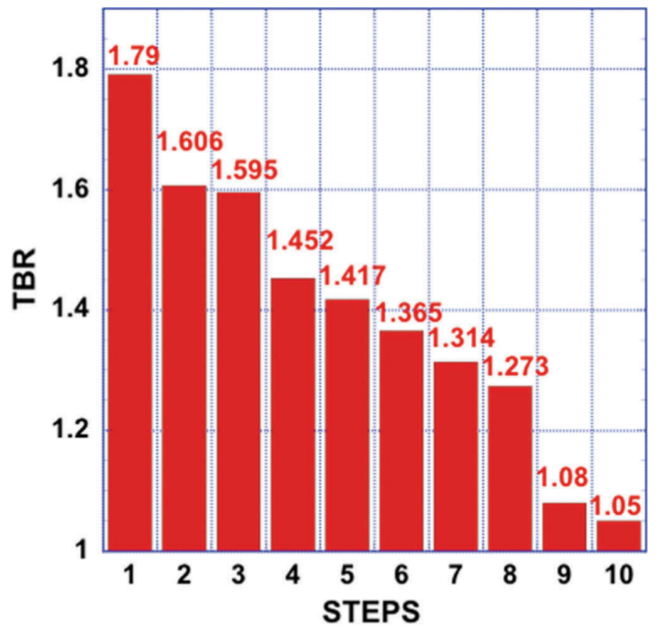
\includegraphics[width=0.48\textwidth]{imgs/aries-act-2-tbr.png}
\caption{\label{fig:aries-act-2-tbr}Impact of heterogeneity and penetrations on system \gls{TBR}.}
\end{wrapfigure}

The objective of this subtask is to provide detailed multi-dimensional nuclear
analysis of a specific fusion energy systems, thus informing its overall
design.  An important consideration for this subtask is to perform the
analysis in a way that allows results to be abstracted beyond any particular
design and inform the design of future systems.  This subtask also includes
the generation of 3-D CAD-based analysis models for use in nuclear analysis as
well as by other \gls{FESS} partners.

One of the primary outcomes of detailed 3-D analysis to identify the peak
magnitudes for various responses, including nuclear heating, dpa and gas
production, within each component.  The material selection and design of each
component is typically based on assessments of those responses from the 1-D
design scoping analysis.  The introduction of heterogeneities and gaps can
have dramatic impact on the local values of those responses even if when it
does not change the average values.  Streaming analysis in ARIES-ACT-1 found
that the damage rates in the inboard structural ring would require replacement
during the lifetime of the system (>200 dpa), but that the both the inboard
and outboard vacuum vessel would survive the entire lifetime of the machine,
although the inboard would not be reweldable.

During this reporting period, a new form of 3-D analysis was implemented to
study the incremental effect of different design elements on the overall
\gls{TBR}.  This analysis provides important guidance for the design process
of future systems in two respects.  First, since 1-D radial builds with
homogenized material compositions are frequently used to iterate over initial
design considerations, it is important to know the degradation in \gls{TBR}
that arises when introducing the realistic heterogeneity of the 3-D structures
that exist within and between components.  Second, it is useful to know how
much degradation in the \gls{TBR} arises from the introduction of each port in
the \gls{FW/B} system.  Fig.\ \ref{fig:aries-act-2-tbr} shows the degradation
in overall \gls{TBR}, in a progression from a fully homogenized inboard and
outboard model to a fully heterogeneous model of many steps.  The final step
shows the impact of penetrations by a simple approximation based on scaling
the first wall area.  A similar analysis on FNSF used full 3-D models to show
similar effects for both penetrations and the addition of the test module
ports.

Nuclear analysis also provides the source term for a variety of thermal
analyses under normal and off-normal conditions.  A 2-D transient thermal
analysis performed by \gls{UW-FTI} during assumed loss of He and water
coolant/loss of LiPb flow conditions found that many components approached
900\ $^\circ$C, suggesting the need for alternate materials.  Detailed 3-D
heating rates were provided to partners for other thermal-structural analysis.

Finally, detailed activation analysis can provide important insight on
\glspl{SDR} and ultimate waste management issues.  Detailed 3-D activation
analysis of ARIES-ACT-1 was used to confirm that the simpler 1-D radial build
analysis is conservative and over-predicts the activation response by up to
30\%.  This supports the continued use of 1-D analysis at this stage of
conceptual design for discussion of waste management.  \gls{SDR} analysis
inherently requires resolving the 3-D distribution of activation photons.  A
detailed \gls{SDR} analysis of FNSF is underway using the \gls{R2S} tools
developed in the previous section, and expected to be completed in summer
2018.

\subsection{Integrated Electromagnetic and Thermal-Structural Analysis}

\begin{wrapfigure}{R}{0.5\textwidth}
\centering
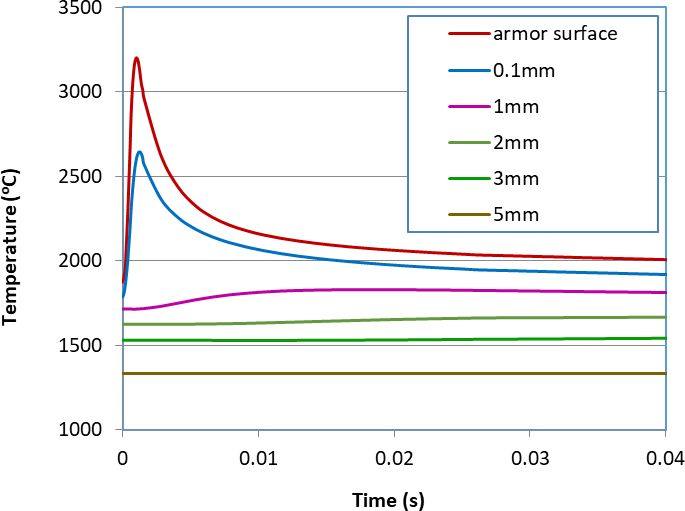
\includegraphics[width=0.48\textwidth]{imgs/elm-thermal.png}
\caption{\label{fig:elm-thermal}Thermal transient in an all-tungsten plate divertor.}
\end{wrapfigure}

The objective of this subtask is to provide detailed multi-dimensional
thermal, mechanical and electromagnetic analysis of specific \glspl{PFC}, thus
informing the design of those components.  This performance period has focused
on solid tungsten and liquid metal \glspl{PFC} exposed to prototypical loads
expected in a tokamak, with consideration for steady heat flux, transient heat
flux (disruptions and \glspl{ELM}), coolant pressure, and electromagnetic
disruption effects.


\subsubsection{Solid Tungsten Surfaces}

\paragraph{Thermo-structural behavior.} Transient thermal behavior is
calculated using commercial finite element codes and temperature-dependent
properties. The structural behavior is more complicated, as it must account
for a numerous nonlinear material behaviors and a variety of failure modes,
including ratchetting and fracture. A typical thermal result is shown in
Fig.\ \ref{fig:elm-thermal}, providing temperature histories during a single
\gls{ELM} pulse in an all-tungsten plate divertor. The primary conclusion from
these analyses is that all-tungsten \glspl{PFC} are probably viable, but
\gls{ELM} control is likely required and improved tungsten-based alloys would
be beneficial. It also identified the importance of thermal creep in these
designs.

\begin{wrapfigure}{R}{0.5\textwidth}
\centering
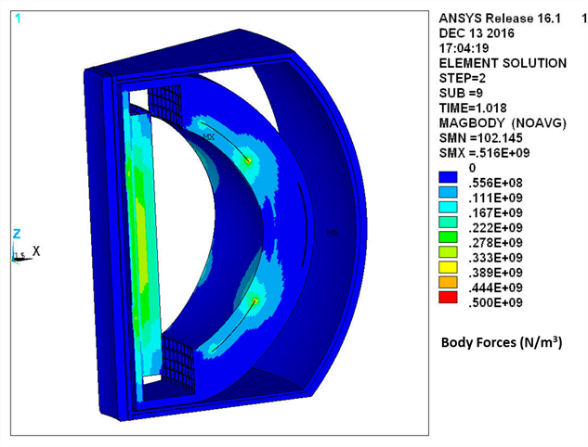
\includegraphics[width=0.48\textwidth]{imgs/disrupt-em.png}
\caption{\label{fig:disrupt-em}Induced body forces on structural components during a disruption.}
\end{wrapfigure}

\paragraph{Electromagnetic effects} Disruptions will induce large loads in
surrounding structures, as a result of induced currents. We have modeled
these, again using commercial finite element codes, assuming plasma quench,
but no plasma motion. Typical results for induced body forces in the key
structures are shown in Fig.\ \ref{fig:disrupt-em}. The key conclusion here is
that disruption forces in FNSF appear to be survivable without significant
damage, though some surface melting is expected from the thermal loads.

\subsubsection{Liquid Surfaces}

\paragraph{Transient thermal behavior.} Thermal transients in liquid surface
\glspl{PFC} are modeled via numerical solution of a partial differential
equation accounting for conduction and energy lost due to evaporation. It is
solved consistently with an evaporation model that relies on temperature
dependent vapor pressure. The heat loads have been calculated using a recent
paper by Kessel, Tillack, and Blanchard. The load is assumed to be a
triangular pulse with a rise time of 1/3 ms and a fall time of 2/3 ms. The peak
fluxes are as high as 1.1 GW/m$^2$ for an \gls{ELM} on a divertor.

\paragraph{Evaporation.} These thermal results are also used to estimate
the mass lost in a single \gls{ELM} pulse. A comparison of the evaporated thickness
for four different liquid metals, assuming an initial temperature of 600K, is
shown below.

The above results assume that the liquid divertor evaporates into a vacuum. In
reality, the situation is much more complicated. One effect that is expected
is vapor shielding, implying that some fraction of the incoming heat flux will
be absorbed in the vapor itself, thus preventing it from reaching the
liquid. This will limit the evaporation possible during a single \gls{ELM}
pulse. The above plots have not accounted for vapor shielding due to the
uncertainties inherent in the calculation. In this sense, the above results
are assumed to be “worst-case” results. We have produced results using a
shielding model akin to transport of the plasma ions through a vapor
cloud. However, these results will be of most value when combined with a model
of the plasma, including a simple core model as well as detailed models of the
edge physics, sheaths, charge exchange, etc. These calculations are
tentatively planned for the coming quarter.

\paragraph{Boiling. } Given that in some cases, the temperatures shown
above exceed the tabulated boiling points for lithium and tin, respectively,
one might be concerned that the mass loss mechanism will be from boiling,
rather than evaporation. This could lead to significant increases in the mass
loss. However, tabulated boiling points do not apply to cases where the
heating is homogeneous and bubbles are nucleated in the bulk. In this case,
the boiling point is substantially higher. A detailed assessment indicates
that boiling is not expected in the cases considered above.

\paragraph{Electromagnetic effects. } Disruptions will induce currents in
a pool-type divertor and the resulting forces could, in principle, empty the
tray. To estimate these forces, we included a static lithium pool-type
divertor in a model of a tokamak and ramped down the plasma current (linearly)
in 18 ms. No plasma motion or halo currents were considered.

The divertor was assumed to consist of a 1 cm thick lithium layer in a 10 cm
thick steel tray (50\% dense). If the divertor is toroidally continuous, then
the induced currents are largely toroidal, but if it is segmented toroidally,
then the current morphology is quite different. Results indicate that a
continuous divertor experiences current densities about 5 times that of a
segmented divertor. Structurally, the divertor tray seems able to withstand
the projected loads, but the liquid will experience very large forces that may
empty the tray. Future calculations will estimate whether retarding forces
induced by the liquid motion are sufficient to keep the liquid in the tray.

\paragraph{Liquid metal embrittlement. } A recent study summarized the
literature on liquid metal embrittlement. This phenomenon represents a
decrease in a metal’s ductility resulting from exposure to liquid metal. The
behavior varies with temperature, grain size, cold work, and stress. The
literature on fusion-relevant solid/liquid couples is limited, but this issue
must be addressed in any liquid metal-based design.

